\chapter{The EASYGL Backend}
\label{ch:easygl-backend}

\texttt{EASYGL} is CNA's default backend on Linux and Emscripten, built on the sibling
\texttt{easy-gl} project introduced in Chapter~\ref{ch:ecosystem-map} and covered as a
project in its own right later in this book. It is also, by the project's own account, the most
mature backend overall --- broadest 3D feature coverage, mostly passing marks across the
entire cross-backend feature matrix.

\section{A documentation staleness warning, taken seriously}

Before any specific claim in this chapter: \texttt{docs/easygl\_bugs.md}, the primary
per-bug record for this backend, carries its own explicit staleness banner. It was last
fully written weeks before this book's own source material was gathered, and states plainly
that it ``has not been re-audited against thousands of lines of EasyGL changes since.'' Only
two of its rows have been independently re-confirmed as fixed; everything else is
``spot-checked, not exhaustively re-verified.'' This chapter treats that banner as
Chapter~\ref{ch:what-is-cna} asked this book to treat every dated claim: reproduced because
it is evidence of real methodology, not because it is guaranteed current.

\section{Confirmed fixed since the original bug list}

Two fixes are independently re-confirmed current: real anisotropic filtering (the requested
\texttt{maxAnisotropy} now genuinely reaches the GPU, gated on the
\texttt{GL\_EXT\_texture\_filter\_anisotropic} extension), and a real, parameterized
\texttt{depthFormat} for cube render targets, replacing what had been a hardcoded
``always has depth'' boolean.

\section{Confirmed pre-existing gaps}

A multi-render-target configuration with more than one attachment leaks the previous
framebuffer object, because unbinding any single render target resets a shared ``MRT ready''
flag regardless of how many targets are actually bound --- the suspected cause of a known,
still-failing MRT test. Separately, an upstream \texttt{easy-gl} GL-state-desync bug (not a
CNA defect) causes one of \texttt{easy-gl}'s own resource smoke tests to fail.

Several platform ceilings are inherent to OpenGL ES~3.0 rather than fixable in CNA at all:
\cnaclass{FillMode::WireFrame} is silently ignored, because GLES3 has no
\texttt{glPolygonMode} to call; \texttt{glDrawElementsBaseVertex} is called unconditionally
without checking for the extension that actually guarantees it (only certain on GLES~3.2,
not the 3.0 baseline this backend otherwise targets) --- on a device lacking the extension,
an indexed draw with a non-zero base vertex can silently render the wrong geometry or crash;
and \cnaclass{OcclusionQuery::PixelCount()} can only ever return 0 or 1 on this driver
profile, because GLES3 exposes only \texttt{GL\_ANY\_SAMPLES\_PASSED}, a boolean visibility
test, not a true sample count.

Two further, real behavioral divergences are documented rather than silently accepted: fog
is computed from clip-space Z rather than true view-space depth, which diverges from XNA at
oblique viewing angles; and \texttt{DrawColoredPrimitives} / \texttt{DrawIndexedColoredPrimitives}
always render through one hardcoded-transform shader program, entirely ignoring whatever
\cnaclass{GpuDrawParams} the effect layer actually supplied.

Missing features confirmed still open include: the \texttt{preserveContents} flag on render
target creation (always behaves as \texttt{DiscardContents}); \texttt{Texture2D::SetData}
uploads never regenerating mipmaps (only the render-target-unbind path does, a separate code
path); \texttt{Texture3D} / \texttt{TextureCube} both ignoring their requested
\cnaclass{SurfaceFormat} (always RGBA8) and their \texttt{mipMap} request; neither type being
registered with the GL-context-loss recovery mechanism the way ordinary 2D textures are;
\texttt{EasyGLEffectBackend::Unbind()} being a pure no-op; \texttt{ApplyBlendState} never
calling \texttt{glColorMask}, so \cnaclass{ColorWriteChannels} has no effect at all; and
\cnaclass{SpriteBatch} carrying a 65{,}535-index limit from its \texttt{uint16\_t} index
type, silently wrapping or corrupting any batch exceeding roughly 16{,}383 quads.
\texttt{VertexBuffer::GetData} / \texttt{IndexBuffer::GetData} have no real per-backend GPU
readback path on this backend, or on any other --- Section~\ref{sec:easygl-getdata-shadow}
below corrects an earlier pass's own overstatement of this gap and explains precisely what
does and does not work.

One gap is formally BLOCKED rather than merely open: forwarding a real, non-\texttt{Color}
\cnaclass{SurfaceFormat} all the way to the GPU conflicts directly with an already-shipped,
already-tested contract on \texttt{Texture::ValidateFormat} (Chapter~\ref{ch:textures-rendertargets})
--- closing this gap would require revisiting a decision the project has already committed
tests against, not simply writing new code.

\subsection{A worked example: finding the real SpriteBatch quad ceiling}

The \texttt{uint16\_t} index-type finding above is worth turning into an actual number, since
``roughly 16{,}383 quads'' is a real, checkable threshold a game can hit without realizing it
if it draws enough distinct sprites inside one \texttt{Begin()} / \texttt{End()} pair (a
particle system, a large tile map batched in one call, a text-heavy UI drawn glyph by glyph):

\begin{lstlisting}
constexpr int kMaxUint16Value = 65535;         // uint16_t's own maximum representable index
constexpr int kVerticesPerQuad = 4;            // one quad = 4 unique vertices, 2 triangles
constexpr int kMaxQuadsBeforeWrap = (kMaxUint16Value + 1) / kVerticesPerQuad; // = 16384
\end{lstlisting}

The one-off discrepancy between this computed 16{,}384 and the chapter's own ``roughly
16{,}383'' figure is itself worth internalizing rather than smoothing over: exactly where the
wraparound first becomes \emph{visibly} corrupt versus merely at its theoretical limit depends
on \cnaclass{SpriteSortMode} and batch-flush timing details this specific finding does not
fully pin down --- treat 16{,}384 as the hard ceiling derived from the index type itself, and
anything close to it as already in the danger zone worth testing directly rather than assuming
safe. A game that might legitimately approach this --- a bullet-hell shooter, a particle-heavy
effect, a very large uniformly-tiled background drawn one \texttt{Draw()} call per tile
instead of one call per texture atlas --- has two real mitigations: split the single
\cnaclass{SpriteBatch} \texttt{Begin()} / \texttt{End()} pair into multiple smaller batches well
under the ceiling, or batch fewer, larger draws (one atlas texture covering many tiles) so the
quad count per batch stays low regardless of how much is actually drawn on screen.

\section{The D3D9 oracle cross-measurement: a genuinely different kind of test}

A separate, one-off investigation ran EasyGL against the same 31-scene oracle corpus built
for the \texttt{D3D9} backend's own pixel-for-pixel verification against real XNA~4.0
(Chapter~\ref{ch:direct3d-backends}). The result: 10 of 31 scenes matched pixel-for-pixel;
21 diverged. This was deliberately \emph{not} promoted to a permanent, ongoing test, because
an EasyGL-versus-real-XNA comparison runs through an entirely different GPU driver stack than
the DXVK-versus-DXVK comparison \texttt{D3D9}'s own oracle performs --- meaning any diff
conflates genuine rendering differences with ordinary driver differences, and cannot cleanly
attribute a mismatch to one or the other. Of the 21 divergent scenes, the investigation
separated three distinct patterns: seventeen were silhouette-edge-only rasterization-convention
differences (an inherent property of any two different GPU rasterizers, not a bug);
two were whole-primitive but imperceptible, 1--2-out-of-255 rounding differences consistent
with ordinary GPU/driver floating-point noise; and two were real, large, whole-primitive
bugs worth naming specifically: a negative-\texttt{FogEnd} configuration rendered as solid
black on EasyGL where D3D9 correctly renders a white-to-black gradient, and an
environment-map Fresnel term failed to interpolate correctly (Gouraud-style) across a
primitive on EasyGL --- a concrete, independent confirmation of a divergence
Chapter~\ref{ch:stock-effects} already predicted from the effect-level audit alone.

\subsection{Both of those two bugs are fixed now --- verified directly against the current shader source}

The investigation's own account (\texttt{docs/d3d9-divergence-report.md}) is explicit that both
findings above were ``logged here, not fixed'' at the time --- but reading
\texttt{EasyGLGraphicsBackend.cpp} directly today shows both have since been closed, and it is
worth correcting the record rather than reproducing a now-stale ``still open'' framing. Every
stock-effect fragment/vertex shader pair in the file carries an identical, explicitly-labeled
comment: ``Task~1111: matches FNA's \texttt{EffectHelpers.SetFogVector} / \texttt{Common.fxh}
\texttt{ComputeFogFactor} exactly \dots{} NOT a naive \texttt{(fogEnd-z)/(fogEnd-fogStart)}
falloff, which silently inverts/collapses once \texttt{FogEnd<FogStart} (oracle scene
\texttt{fog\_gradient\_quad})'' --- naming the exact failing scene from the cross-measurement
above by name. Working the corrected formula through with the oracle scene's own real values
(\texttt{FogStart=0}, \texttt{FogEnd=-1}) confirms the fix is not just labeled correctly but
mathematically sound: \texttt{vFogFactor = clamp((z + FogEnd) / (FogEnd - FogStart), 0, 1)}
becomes \texttt{(z - 1) / (-1) = 1 - z} at these values, giving \texttt{vFogFactor = 1} (fully
unfogged, original color shows through) at the near edge $z=0$ and \texttt{vFogFactor = 0}
(fully fogged) at the far edge $z=1$ --- exactly the near-white-to-near-black gradient real XNA
renders, not the solid-black collapse the pre-fix naive formula produced. The Fresnel bug has
an equally explicit fix comment, a few hundred lines later in the same file, labeled
Task~1112: the vertex shader now computes \texttt{viewAngle} from \emph{each vertex's own
un-interpolated} normal and eye vector before the Fresnel \texttt{pow()} term is evaluated, so
the GPU's own Gouraud interpolation happens to the already-computed scalar afterward --- matching
real XNA's \texttt{EnvironmentMapEffect.fx} exactly, rather than the mathematically distinct
operation of interpolating the normal first and recomputing Fresnel per fragment. Both fixes
apply uniformly across every one of this backend's stock-effect shader programs (colored,
textured, color-plus-textured, and the lit/skinned variants alike), not as a one-off patch to
the single scene that exposed each bug.

\section{A second stale-doc claim, this time about \texttt{Viewport}}

The staleness warning this chapter opened with applies to more than just
\texttt{docs/easygl\_bugs.md}. \texttt{docs/rendertarget-support.md} --- the same document
Chapter~\ref{ch:vulkan-backend}'s own equivalent finding drew from, where three of its own
tracked tasks turned out to already be fixed on Vulkan --- lists this backend's own
\texttt{Viewport} support identically: ``zero wiring on any backend'' (Task~880), meaning a
custom sub-region \cnaclass{Viewport} was believed to have no actual GPU effect at all.
Reading \texttt{EasyGLGraphicsBackend.cpp} directly instead of trusting that status column
finds the same Task~880 fix already landed here too, with real, unconditional
\texttt{device.set\_viewport()} / \texttt{device.set\_depth\_range()} calls replacing whatever
no-op previously sat behind \texttt{SetViewport()}.

The comparison with Vulkan's own version of this exact fix (Chapter~\ref{ch:vulkan-backend})
is worth drawing out, because the two backends did not land at the same scope. Vulkan's fix is
honestly limited to the backbuffer pass only --- a render-target pass there stays hardcoded to
that target's own full size, because Vulkan's deferred, once-per-frame command-recording model
has no way to recover which \cnaclass{Viewport} was active at the moment a given render
target's draws were originally issued. EasyGL has no equivalent limitation, for an
architectural reason rather than extra effort spent on this specific fix: \texttt{SetViewport()}
issues its OpenGL calls immediately, at the moment a game actually calls it, with no deferred
recording step in between --- so the same fix genuinely applies whether or not a
\cnaclass{RenderTarget2D} / \cnaclass{RenderTargetCube} face is currently bound, using the active
target's own height (\texttt{currentRtHeight\_}) for the coordinate-origin flip instead of the
window's physical height whenever one is. A concrete illustration of a theme
Chapter~\ref{ch:backend-architecture} already introduced in the abstract: two backends
implementing the identical interface method can genuinely differ in how completely they can
honor it, for reasons rooted in each backend's own underlying execution model rather than in
how carefully either one was built.

\subsection{A claim this chapter itself got wrong: two-sided stencil's shared mask is correct, not a bug}

An earlier pass of this chapter listed ``two-sided stencil incorrectly reusing the front-face
read mask for the back face too'' among this backend's confirmed gaps. Reading
\texttt{ApplyDepthStencilState()} in \texttt{EasyGLGraphicsBackend.cpp} directly shows exactly
that: the function's \texttt{Back}-face call to
\texttt{set\_stencil\_func\_separate()} passes the same \texttt{stencilMask} local
variable the \texttt{Front}-face call already used, with no separate
back-face mask value anywhere in the function:

\begin{lstlisting}
device.set_stencil_func_separate(::easygl::CullFace::Front,
    ToEasyGLCompareFunc(stencilFunc),
    referenceStencil, static_cast<unsigned int>(stencilMask));
// ...
// Back-face call below passes the same stencilMask -- not a separate ccw one.
device.set_stencil_func_separate(::easygl::CullFace::Back,
    ToEasyGLCompareFunc(ccwStencilFunc),
    referenceStencil, static_cast<unsigned int>(stencilMask));
\end{lstlisting}

The claim that this is \emph{incorrect} does not survive checking real XNA's own documented
contract before assuming CNA's own code is at fault --- exactly the discipline
Chapter~\ref{ch:what-is-cna} asks every claim in this book to meet. \texttt{xna4-spec}'s own
\texttt{DepthStencilState.xml} defines four separate \cnaclass{CounterClockwiseStencil}*
properties (\texttt{Function}, \texttt{Fail}, \texttt{DepthBufferFail}, \texttt{Pass} --- all
four genuinely \emph{operations}) but exactly one \texttt{StencilMask} property, with no
\texttt{CounterClockwiseStencilMask} anywhere in the type at all. Real XNA 4.0 itself has no API
surface for a separate back-face stencil mask to begin with --- a game targeting real XNA cannot
set one, so a backend cannot fail to honor a value that was never settable in the first place.
Reusing \texttt{stencilMask} for both faces is not a shortcut standing in for a missing feature;
it is the \emph{only} behavior consistent with the real, documented API this class faithfully
reproduces, confirmed by the same pattern for \texttt{stencilWriteMask} a few lines later in the
identical function (also passed unchanged to both \texttt{Front} and \texttt{Back}, and also
correctly so --- real XNA's \texttt{StencilWriteMask} is likewise a single, non-per-face
property).

What genuinely \emph{is} per-face, and what this same function gets right, is worth stating
precisely rather than lumping the whole feature together as either ``correct'' or ``buggy'':
the four \cnaclass{CounterClockwiseStencil}* \emph{operation} properties are threaded through
as \texttt{ccwStencilFunc} / \texttt{ccwStencilFail} / \texttt{ccwStencilDepthFail}/%
\texttt{ccwStencilPass}, distinct parameters from their clockwise counterparts, and applied to
\texttt{CullFace::Back} via a genuinely separate \texttt{set\_stencil\_op\_separate()} call ---
real per-face divergent behavior, exactly where real XNA's own API allows it to diverge. A
mirror-reflection technique relying on \texttt{TwoSidedStencilMode} (the same worked example
Chapter~\ref{ch:state-objects} builds around \cnaclass{DepthStencilState}) can safely assume
different \emph{stencil operations} for front- and back-facing geometry on this backend, but
must not assume a different \emph{stencil mask} is possible for either face --- not a
limitation of this backend specifically, but of the real XNA type every backend implements
identically.

\section{\texttt{GetData()} really does work --- just not the way ``no GPU readback'' implies}
\label{sec:easygl-getdata-shadow}

An earlier pass of this chapter said \cnaclass{VertexBuffer} / \cnaclass{IndexBuffer}
\texttt{GetData} were ``not implemented at all'' on this backend, with ``no interface method
to even express a readback request.'' Reading \texttt{VertexBuffer.hpp} / \texttt{.cpp} directly
shows that framing overstates the gap: \texttt{GetData} is real, public API, and it genuinely
returns correct data --- it is just never a GPU readback at all, on \emph{any} backend,
because it does not need to be. A private \texttt{cpuShadow\_} byte buffer, declared directly
on \cnaclass{VertexBuffer} itself (not per-backend), caches every \texttt{SetData} call's
already-packed GPU-layout bytes:

\begin{lstlisting}
// Task 930: CPU-side shadow of the most recent SetData call's compact GPU-layout
// bytes, enabling GetData() without a real per-backend GPU readback path (mirrors
// Texture2D's own SetData/GetData shadow-buffer precedent) -- nothing in the XNA
// 4.0 pipeline writes back into a VertexBuffer from the GPU side, so a CPU shadow
// is a fully faithful implementation, not an approximation.
std::vector<std::uint8_t> cpuShadow_;
\end{lstlisting}

The comment's own justification is worth taking at face value rather than treating the shadow
as a stopgap: real XNA's \cnaclass{VertexBuffer} / \cnaclass{IndexBuffer} are never written to
by the GPU pipeline (no compute shaders, no transform feedback in the XNA 4.0 model), so
\texttt{SetData} followed by \texttt{GetData} is a round-trip through CPU memory in real XNA
too --- a CPU shadow is not an emulation of a missing capability, it is the same shape real
XNA's own contract already has. \texttt{IndexBuffer} carries the identical mechanism, confirmed
by its own header comment pointing back to \cnaclass{VertexBuffer}'s as the shared rationale.
Both throw \texttt{NotSupportedException} correctly when \texttt{GetData} is called on a
\texttt{BufferUsage::WriteOnly} buffer, matching real XNA's own documented restriction --- the
shadow exists but is deliberately not consulted in that case.

There is one shared typed-path exception this chapter's earlier wording missed:
the options-taking \texttt{SetData} wrappers on both dynamic buffer classes upload correctly
but never refresh their public \texttt{cpuShadow\_} vectors. With
\texttt{BufferUsage::None}, an inherited \texttt{GetData} after that normal dynamic upload
sees an empty or stale shadow; this fails identically on every backend and is not an EasyGL
readback limitation. Chapter~\ref{ch:textures-rendertargets} traces the exact path.

\subsection{The separate raw-layout gap: \texttt{SetDataRaw}}

Chapter~\ref{ch:backend-architecture}'s Task~1080 custom-vertex-layout capability --- EasyGL's
own extension letting a caller supply an arbitrary \cnaclass{VertexDeclaration} instead of only
the five stock \texttt{VertexPositionXxx} types --- reaches the backend through a different,
\texttt{NOXNA} entry point, \texttt{SetDataRaw()}, and that path does \emph{not} participate in
the shadow mechanism at all:

\begin{lstlisting}
void VertexBuffer::SetDataRaw(const void* data, int count, int stride)
{
    if (getIsDisposedProperty())
        throw System::ObjectDisposedException("VertexBuffer");
    backend_->SetVertexDeclaration(vertexDeclaration_.GetVertexElements());
    backend_->SetData(data, count, static_cast<std::size_t>(stride));
    // No cpuShadow_ update here -- unlike every typed SetData(VertexPositionXxx*, ...)
    // overload above.
}
\end{lstlisting}

\texttt{GetData} itself is only ever declared for the five stock types, so there is no
\texttt{GetDataRaw} counterpart to call after a custom-layout upload in the first place --- a
caller who populates a buffer through \texttt{SetDataRaw()} and then genuinely needs the data
back has no API surface to ask with at all, typed or raw. This is a narrower, more precisely
scoped gap than the earlier ``not implemented at all'' framing suggested: ordinary XNA-shaped
vertex data uploaded through the ordinary non-options overloads round-trips correctly through
\texttt{GetData} on this backend exactly like every other one. The \texttt{NOXNA}
custom-layout extension has no raw readback surface at all, while the separate dynamic-options
shadow bug above affects typed data project-wide.

\section{Test baseline}

The feature matrix records exactly three known pre-existing test failures for this backend:
the two-attachment MRT test, a reference-stencil test, and the upstream \texttt{easy-gl}
resource smoke-test issue already covered above --- against a full suite exceeding 4{,}500
tests overall, giving a sense of how narrow the genuinely open surface is relative to the
backend's total scope.

\section{A real screenshot, captured headlessly under Xvfb}

\texttt{EASYGL} opens a real SDL3 window and issues real OpenGL ES calls, so --- unlike the
\texttt{SOFTWARE} backend's screenshots elsewhere in this book, reachable with no display at
all --- a genuine screenshot needs a genuine (if virtual) display. This book's own
screenshot-feasibility notes named \texttt{Xvfb} plus Mesa's software \texttt{llvmpipe} GL
implementation as plausible for exactly this case, but had explicitly left it untested.

Building this backend with \texttt{CNA\_BUILD\_EXAMPLES=ON} and running a small headless demo
under \texttt{xvfb-run} confirms the technique works here too, using the identical scene and
capture helper as Chapter~\ref{ch:sdl-renderer}'s own equivalent section: the real
\texttt{examples/easygl\_spritebatch\_rotation\_golden\_test.cpp} rotate-around-origin scene
(Task~465/417; also Chapter~\ref{ch:spritebatch}'s own worked example), captured via
\texttt{SaveBackBufferScreenshotEXT} after \texttt{xvfb-run -a --server-args="-screen 0
1024x768x24" env -u WAYLAND\_DISPLAY ./build-easygl/cna\_xvfb\_screenshot\_demo\_easygl}.

\begin{figure}[h]
\centering
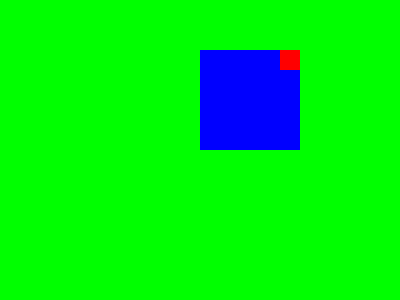
\includegraphics[width=0.5\textwidth]{images/ch18-spritebatch-rotation-easygl.png}
\caption{Real, unedited output of the same rotate-around-origin \cnaclass{SpriteBatch} scene as
Figure~\ref{fig:ch17-spritebatch-rotation}, this time rendered by \texttt{EASYGL} through a real
OpenGL ES context under a virtual \texttt{Xvfb} display. The two images are pixel-identical for
this scene --- a real, independent cross-backend agreement on a case both backends' own audits
(this chapter's Phase~1111/1112 fixes; Chapter~\ref{ch:sdl-renderer}'s Phase~70 audit) already
established each gets right on its own.}
\label{fig:ch18-spritebatch-rotation}
\end{figure}

Figure~\ref{fig:ch18-spritebatch-rotation} is that real output. Confirming both backends
produce the same result for the same scene is a small but genuine independent data point: it is
exactly the kind of pixel-level cross-backend agreement the D3D9 oracle corpus elsewhere in this
chapter measures far more systematically, here obtained by the simplest possible
means --- two real screenshots, compared by eye.
